%!TEX root=main.tex

\subsection{Algoritmos}

\subsubsection{Minmax}

Quando o jogador computador tem que efetuar uma jogada, o algoritmo Minmax determina quais as jogadas possíveis. Cada uma destas jogadas é analisada da seguinte forma:
\begin{itemize}
	\item se tiver sido atingido o nível de profundidade especificado para o algoritmo, é calculado um valor para o tabuleiro, usando uma heurística do ponto de vista do computador;
	\item se a jogada conduzir ao final do jogo, é atribuído um valor ao tabuleiro tendo em conta quem ganhou, isto é, $+\infty$ se ganha o computador, $-\infty$ se ganha o adversário, $0$ em caso de empate;
	\item se nenhuma das condições anteriores se verificar, são calculadas todas as jogadas seguintes possíveis e o processo repete-se.
\end{itemize}
Para determinar o valor da jogada original (a decisão que o computador tem que tomar no momento), entra a parte do Minmax propriamente dita:
\begin{itemize}
	\item se for a vez do adversário, o valor do tabuleiro é o mínimo dos valores das possíveis jogadas seguintes;
	\item se for a vez do computador, o valor do tabuleiro é o máximo dos valores das possíveis jogadas seguintes.
\end{itemize}

A ideia é bastante simples, dado que assumimos que o adversário fará o melhor para ele, ou seja o pior para o computador e, portanto, escolherá a jogada com um valor mínimo do ponto de vista do computador. Por outro lado, o computador a cada passo escolhe a jogada com um valor máximo para si, o que também faz todo o sentido.

\subsubsection{Minmax Alfa-Beta}

Para melhorar a eficiência do algoritmo Minmax, em termos temporais, utilizam-se cortes Alfa-Beta, que cortam ramos da árvore de decisão cuja análise é desnecessária. Em cada nó da árvore, calculam-se valores $\alpha$ e $\beta$:
\begin{itemize}
	\item $\alpha$ é o melhor valor já encontrado para o maximizador desde esse nó até à raiz;
	\item $\beta$ é o melhor valor já encontrado para o minimizador desde esse nó até à raiz.
\end{itemize}
Nos nós maximizadores atualiza-se $\alpha$ se um dos seus nós filhos apresenta maior valor que o $\alpha$ atual. Nos nós minimizadores atualiza-se $\beta$ se um dos seus nós filhos apresenta menor valor que o $\beta$ atual. Sempre que $\alpha \geq \beta$ efetuamos uma poda, isto é, não continuamos com a análise desses ramos da árvore, porque já sabemos que não apresentarão resultados que nos interessem. 

\subsubsection{Minmax Alfa-Beta Delimitado}

Este é um algoritmo consiste a adição de uma modificação ao algoritmo original de Alfa-Beta. Nele é possível definir um limite máximo e mínimo. Quando um nodo do tipo Max encontra um valor superior ao limite máximo ou um nodo do tipo  encontra um valor inferior ao limite mínimo considera-se que se encontrou uma solução suficientemente boa, não se visitando possíveis jogadas ainda visitadas num determinado nodo.

Com esta abordagem podemos facilmente cortar nós após um nodo encontrar uma jogada vencedora pois o valor de utilidade atribuído a estes tabuleiros é muito superior ao obtido, geralmente, pelas heurísticas. Além disso também é possível usar um Minmax mais flexível, que tenha mais consideração pela performance temporal em detrimento da precisão do resultado obtido.

\subsection{Funcionalidades e Otimizações}

\subsubsection{Generalização para múltiplas jogadas}

Os algoritmos implementados permitem a realização de vários movimentos (sub-jogadas) por um jogador, o que é um detalhe crítico no Pentago cuja vitória pode ser alcançada após o colocar de uma peça sem se realizar a rotação dos quadrantes. Detalhes da implementação são mencionados na secção~\ref{subjogadas_estrutura} deste relatório.

\subsubsection{Remoção de duplicados}

A fim de tentar melhorar a performance temporal são identificados e descartados tabuleiros iguais quando são efetuadas rotações de quadrantes dentro do Minmax. 

Esta verificação compara todas as posições dos tabuleiros. Provavelmente não constitui a solução mais eficaz. Nesse sentido a representação de 72 bits parece mais tentadora. Claro que  também teria algum processamento adicional devido na realização de rotações. Uma vez que não foi usada não podemos tirar conclusões sobre esta alternativa. 

Dos testes de eficiência temporal usados esta modificação apenas é benéfica em tabuleiros com poucas peças, perdendo a sua eficiência quando usada com tabuleiros com mais de 7 peças aproximadamente. A partir de 7 peças, para a maioria dos tabuleiros, a eficiência temporal com remoção de duplicados é pior do que aquela sem remoção de duplicados. No entanto, mesmo nestes casos, a perda de eficiência provocada não é substancial, pelo menos para as profundidades usadas no projeto.

\subsubsection{Simetrias}

O Pentago é um jogo particularmente interessante do ponto de vista das simetrias. O grupo de simetrias do Pentago é o grupo diedral $D_4$, que tem 8 elementos:
\begin{itemize}
	\item o elemento neutro ou identidade;
	\item 3 rotações, de 90, 180 e 270 graus centígrados;
	\item 4 reflexões, horizontal, vertical e duas diagonais.
\end{itemize}

Além destas simetrias, por vezes é ainda útil considerar simetrias de cada quadrante. De facto, o grupo de simetrias de cada quadrante é também $D_4$, mas nós apenas consideramos as reflexões na diagonal principal do primeiro quadrante. 

É de notar que quando o tabuleiro é simétrico relativamente à rotação de $90^{\circ}$ também é simétrico relativamente às rotações de $180^{\circ}$ e de $270^{\circ}$. Além disso, há várias composições de transformações cujo resultado implica outras transformações. Por exemplo, se tiver simetria de reflexão vertical e simetria de reflexão horizontal, então também tem simetria de rotação de $180^{\circ}$. Isto permite evitar verificações desnecessárias de simetrias. 

O algoritmo utilizado para validar simetrias é o que se apresenta a seguir.
\begin{enumerate}
	\item O tabuleiro é simétrico relativamente à rotação de $180^{\circ}$.
		\begin{enumerate}
			\item O tabuleiro é simétrico relativamente à rotação de $90^{\circ}$.
			\begin{enumerate}
				\item O primeiro quadrante é simétrico relativamente à sua diagonal principal. Então basta explorar as próximas jogadas nos nós acima da diagonal principal do primeiro quadrante.
\begin{table}[H]
\centering
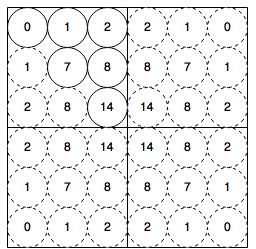
\includegraphics[height=4cm]{images/p180_90_dp0.png}
\end{table}			
				\item O primeiro quadrante não é simétrico relativamente à sua diagonal principal. Então basta explorar as próximas jogadas nos nós do primeiro quadrante.
\begin{table}[H]
\centering
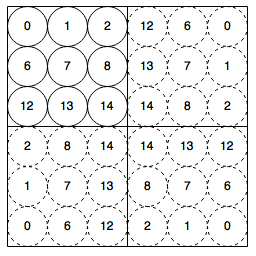
\includegraphics[height=4cm]{images/p180_90.png}
\end{table}			
			\end{enumerate}
			\item O tabuleiro não é simétrico relativamente à rotação de $90^{\circ}$, mas é simétrico relativamente à reflexão vertical.
			\begin{enumerate}
				\item O primeiro quadrante é simétrico relativamente à sua diagonal principal. Então basta explorar as próximas jogadas nos nós acima da diagonal principal do primeiro quadrante.
\begin{table}[H]
\centering
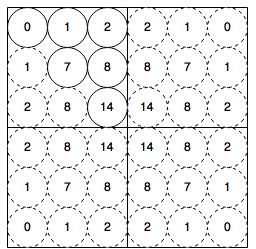
\includegraphics[height=4cm]{images/p180_rv_dp0.png}
\end{table}			
				\item O primeiro quadrante não é simétrico relativamente à sua diagonal principal. Então basta explorar as próximas jogadas nos nós do primeiro quadrante.
\begin{table}[H]
\centering
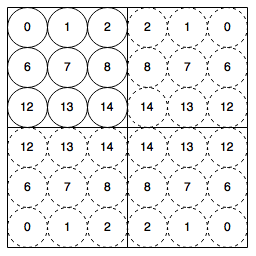
\includegraphics[height=4cm]{images/p180_rv.png}
\end{table}			
			\end{enumerate}
			\item O tabuleiro não é simétrico relativamente à rotação de $90^{\circ}$, nem é relativamente à reflexão vertical, mas é simétrico relativamente à reflexão na diagonal principal. Então basta explorar as próximas jogadas no \emph{triangulo superior}.
\begin{table}[H]
\centering
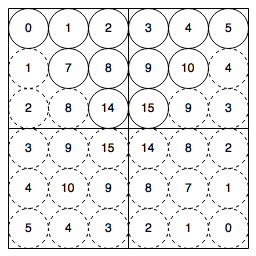
\includegraphics[height=4cm]{images/p180_dp.png}
\end{table}			
			\item O tabuleiro não é simétrico relativamente à rotação de $90^{\circ}$, nem é relativamente à reflexão vertical, nem relativamente à reflexão na diagonal principal. Então basta explorar as próximas jogadas nos nós dos dois primeiros quadrantes.
\begin{table}[H]
\centering
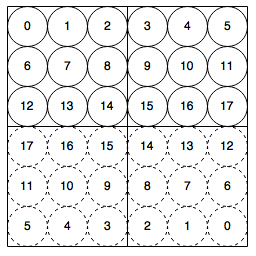
\includegraphics[height=4cm]{images/p180.png}
\end{table}			
		\end{enumerate}
	\item O tabuleiro não é simétrico relativamente à rotação de $180^{\circ}$.		
		\begin{enumerate}
			\item O tabuleiro é simétrico relativamente à reflexão vertical. Então basta explorar as próximas jogadas nos nós dos dois primeiros quadrantes.
\begin{table}[H]
\centering
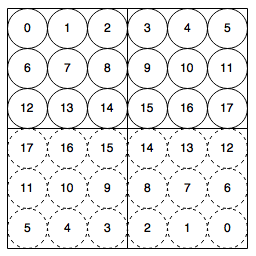
\includegraphics[height=4cm]{images/p_rv.png}
\end{table}
			\item O tabuleiro não é simétrico relativamente à reflexão vertical, mas é simétrico relativamente à reflexão horizontal. Então basta explorar as próximas jogadas no primeiro e no terceiro quadrantes.
\begin{table}[H]
\centering
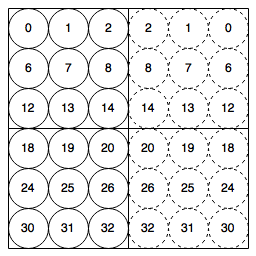
\includegraphics[height=4cm]{images/p_rh.png}
\end{table}			
			\item O tabuleiro não é simétrico relativamente à reflexão vertical, nem relativamente à reflexão horizontal, mas é simétrico relativamente à reflexão na diagonal principal. Então basta explorar as próximas jogadas acima da diagonal principal.
\begin{table}[H]
\centering
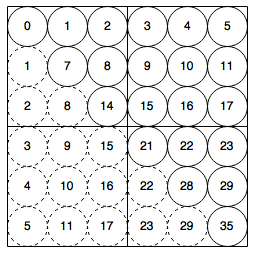
\includegraphics[height=4cm]{images/p_dp.png}
\end{table}			
			\item O tabuleiro não é simétrico relativamente à reflexão vertical, nem relativamente à reflexão horizontal, nem relativamente à reflexão na diagonal principal, mas é simétrico relativamente à reflexão na anti diagonal. Então basta explorar as próximas jogadas acima da anti diagonal.
\begin{table}[H]
\centering
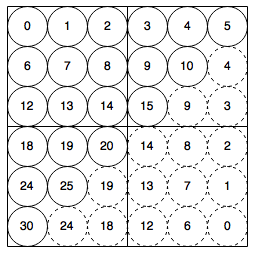
\includegraphics[height=4cm]{images/p_ad.png}
\end{table}			
		\end{enumerate}
\end{enumerate}

Uma vez que apenas podem existir simetrias acontecer quando o número de peças no tabuleiro é par, para agilizar o processamento, apenas verificamos as simetrias nesta situação. Quando o número de peças no tabuleiro é muito reduzido, a verificação de simetrias introduz melhorias significativas. Uma vez perante um número de peças maior os resultados são significativamente piores. Na versão final do projeto, foi colocada uma restrição para apenas ser efetuada validação de simetrias para tabuleiros com um número de peças reduzido. Esta restrição está em vigor nos testes de eficiência temporal apresentados.

\subsubsection{Profundidade Automática}

Ao aumentar o número de peças de um tabuleiro o número médio de nodos filho a analisar por cada nodo no Minmax diminui. Assim é possível analisar a uma profundidade mais elevada,  mantendo (aproximadamente) o mesmo tempo de execução. As profundidades usadas automaticamente face ao número de peças foram escolhidas de acordo com palpites educados, calculando o número aproximado de nós a serem visitados, sendo depois realizados ajustes manualmente após a realização de testes de eficiência temporal. Por prevenção foi dada alguma margem de erro, isto é, algumas profundidades podiam ser aplicadas com um maior número de peças no tabuleiro do que aquele que está estabelecido no código.